\documentclass[14pt]{beamer}
%\usetheme{Singapore}
\usecolortheme{ietf93color}
\setbeamerfont{page number in head/foot}{size=\large}
\setbeamertemplate{footline}[frame number]
\setbeamertemplate{navigation symbols}{}

\mode<presentation>
\title{IPV6 Destination/Source Routing}
\subtitle{%
  draft-lamparter-rtgwg-dst-src-routing-01%
}
\author{%
  \underline{David Lamparter}%
}
\date{IETF 93, July 2015, Prague}
\begin{document}

\begin{frame}
  \titlepage
\end{frame}

\begin{frame}
  \frametitle{Context refresher}
  \begin{itemize}
  \item homenet multiple uplinks vs. BCP 38 filtering\\%
    cf. draft-baker-rtgwg-src-dst-routing-use-cases (IETF88)
  \item draft-baker-ipv6-ospf-dst-src-routing (exp) \&\\%
    draft-baker-ipv6-isis-dst-src-routing\\%
    overlap in describing forwarding behaviour
  \item implementations exists
    (HNCP, BABEL \& IS-IS control planes, Linux kernel forwarding)
  \end{itemize}
\end{frame}

\begin{frame}
  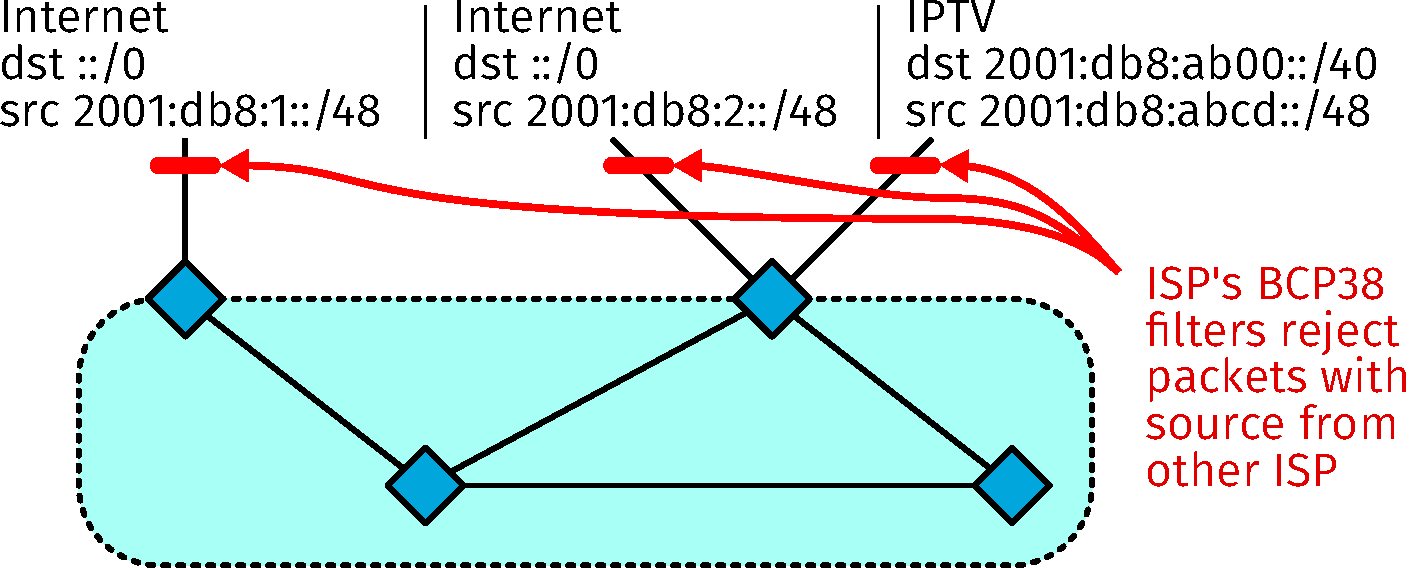
\includegraphics[scale=0.45,angle=0]{intro_topo_bcp.pdf}%
\end{frame}

\begin{frame}
  \frametitle{Changes since -00}

  Dropped ``extra qualifiers'' stuff.

  \vspace{5mm}

  No longer trying to create a generic framework for people changing the
  longest prefix match function.

  \vspace{3mm}

  Simply adding source LPM ``after'' dest LPM.

  \vspace{5mm}

  {\footnotesize No more flowlabels in LPM}
\end{frame}

\begin{frame}
\frametitle{Lookup behaviour}
A route with longer destination prefix match is always more specific than
any other route with shorter destination prefix match, regardless of any source
prefixes.

\vspace{5mm}

Only between the \underline{\color{red}same} destination prefix, source
prefixes are longest-matched.

\vspace{5mm}

Route that doesn't match both is not a match.
\end{frame}

\begin{frame}
\frametitle{Lookup behaviour}
draft specifies \underline{\color{red}continuing to less specific destination} matches
if no entry produces a source match\\
(i.e. modeled as one integral lookup process, not 2 separate steps)\\[1cm]
This is noted as general principle -- stopping lookup can always be done
by inserting an unreachable or blackhole route.
\end{frame}

\begin{frame}
\frametitle{Lookup behaviour}
\includegraphics<1>[width=95mm,angle=0]{ietf_93_lookup_without_ur.pdf}%
\includegraphics<2>[width=95mm,angle=0]{ietf_93_lookup_with_ur.pdf}%

\vspace{3mm}

\only<1>{\small Not allowed to give up after step \#2}
\only<2>{\small Route \#3 must be explicitly installed if ``give up'' desired}
\end{frame}

\begin{frame}
  \frametitle{Open topics: recursive routes}

  Most dst-src work happened in homenet -- little concern given to interop
  with non-homenet.\\[5mm]
  \begin{itemize}
    \item Recursive routes where nexthop matches D/S route
    \begin{itemize}
      \item 2001:db8::/32 via 2001:db8:abcd::1 recursive
      \item 2001:db8:abcd::/48 src 2001:db8:1234::/48 via A
      \item 2001:db8:abcd::/48 src 2001:db8:5678::/48 via B
    \end{itemize}
    \item questionable relevance?
    \item multiple routes installed?
  \end{itemize}
\end{frame}

\begin{frame}
  \frametitle{Other integration concerns}

  Unicast RPF:
  \begin{itemize}
    \item Filtering incoming packets based on route lookup with dst and src reversed
    \item previously: only check packet src $\Leftrightarrow$ route dst
    \item draft says: allowed to ignore packet dst, or also check packet dst $\Leftrightarrow$ route src
  \end{itemize}
  \vspace{5mm}
  Multicast RPF:
  \begin{itemize}
    \item MRPF only ever uses multicast sender address
    \item draft says: ``ignore D/S routes, not applicable''
    \item proper solution: separate multicast topology
  \end{itemize}
\end{frame}

\begin{frame}
  \frametitle{Next steps}
  \begin{itemize}
    \item looking to get this adopted as rtgwg WG document
    \item homenet WG needs this
    \begin{itemize}
      \item independent of / applies to all choices of routing protocol
    \end{itemize}
    \item have personally seen use case in service provider network
       (user class $\Rightarrow$ BGP peers mapping)
  \end{itemize}
\end{frame}

\end{document}
